\chapter{声学分形拓扑模型的有限元仿真和实验观测}
\section{引言}
拓扑物理在近年来成为凝聚态物理和材料科学的研究热点,其中霍尔丹模型因其能够在无外磁场的情况下展现拓扑非平庸能带结构而备受关注。霍尔丹模型的核心特征在于其包含虚时反对称跃迁项,从而实现量子反常霍尔效应。然而,在经典尺度或实验实现中,该模型的推广仍然面临挑战,特别是在复杂结构、有限尺寸效应及边界态稳定性等方面的探索仍处于发展阶段。

最近的理论研究表明,拓扑态甚至可以超越整数维度,存在于分形晶格中\cite{song2014topological,pai2019topological,iliasov2020hall,fremling2020existence,yang2020photonic,ivaki2022topological}。分形几何与拓扑物理的结合提供了一种新的研究范式。分形在不同尺度上表现出相同的特征,具有分形维度、自相似性和尺度不变性\cite{Mandelbrot1982,gouyet1997physics}。分形结构因其自相似性和多尺度特性,在电子、光学以及声学系统中均展现出独特的物理性质。它们不像整数维晶体那样具有明确的体态,但仍然能够支持拓扑边缘态。尽管对拓扑分形绝缘体的兴趣日益增加,但实验实现并不简单,早期的尝试\cite{liu2021sierpinski}表明,分形特性可能会关闭拓扑性质。直到最近,有报道称在由螺旋波导组成的Sierpinski光子分形晶格中实现了Floquet拓扑态\cite{yang2020photonic,biesenthal2022fractal}。这些在凝聚态物理和光子学领域的进展改变了当前对体-边对应关系的理解:拓扑性质不一定依赖于内部体态。然而,迄今为止,拓扑分形物理学的实验验证仍然很少,拓扑相图与分形特性之间的相互作用仍然知之甚少。将霍尔丹模型与BBH模型推广到分形系统,不仅可以揭示拓扑态在非整数维度空间中的行为,还能为拓扑物理与分形科学的交叉研究提供新的思路。

本章主要研究声学分形拓扑模型的有限元方法(Finite Element Method, FEM)仿真及实验观测。本章涉及两个模型:谢宾斯基三角形上的霍尔丹模型与谢宾斯基地毯上的BBH模型。

首先,我们基于有限元方法构建分形几何中的霍尔丹模型,通过求解声学原胞在周期性边界条件和声学分形霍尔丹模型的频谱,分析了其能带和拓扑性质。随后,我们通过实验手段验证该模型的可行性。声学分形晶格通过3D打印技术构建,通过一个特定频率的相位阵列激发了系统的声学拓扑态。

接下来,我们通过实验在声学分形晶格中展示了一种新的高阶拓扑相,从而提供了一种新的范式。通过在方形晶格中引入分形性,我们揭示了一个受限的高阶相位图,其中包含丰富的角态,包括零维外角态和 1.89 维内角态。因此,该系统的余维数为 1.89,该分形模型可归类为分数阶拓扑绝缘体。角态的分数维度此前从未被报道,因此使得我们的研究与传统拓扑绝缘体明显不同。在一个制备的分形晶格中,我们通过局部声学测量实验观察到了外/内角态。

我们的研究展示了声学分形晶格中的一阶和高阶拓扑相,并可能为分数阶拓扑绝缘体的发展铺平道路。研究结果将有助于加深对分形拓扑物理的理解,并为拓扑电子学、光子学及其他领域提供启发。

\section{分形霍尔丹模型的有限元仿真}
\subsection{三维Weyl点与二维霍尔丹模型的有效映射}
我们的分形系统可以从拓扑 霍尔丹 模型的声学版本构建。声波本身不对磁场作出反应,因此实现霍尔丹模型的难点在于实现其原胞内交错的磁场。因此实验的关键在于实现一个合适的复次近邻耦合,诱发出霍尔丹模型的交错等效磁场。本文采用Meng Xiao等人在2015年提出的方案\cite{xiao2015synthetic},利用第三维的手性管道提供复次近邻耦合和合成规范场。该模型是一个三维的Weyl半金属(Weyl semimetal),霍尔丹模型是其在二维的有效映射。

Weyl半金属是具有Weyl点的材料\cite{wan2011topological}。 Weyl 半金属在三维动量空间中承载孤立的 Weyl 点,这些 Weyl 点已在 TaAs 材料\cite{lv2015experimental,xu2015discovery} ,双旋光子晶体\cite{lu2015experimental}和声学系统\cite{li2018weyl,ge2018experimental}中被发现。 Weyl 材料表现出新奇的物理性质,例如开放的费米弧\cite{wan2011topological}和手性异常\cite{nielsen1983adler}。新兴的 Weyl 物理学在凝聚态物理,光子学领域和声学领域引起了广泛关注。

Weyl点的基本理论来源于Weyl方程,该方程描述了无质量的费米子粒子, 由 Weyl 哈密顿量\cite{weyl1929electron}描述:
\begin{equation}
H(\mathbf{k}) = \sum_{i,j=x,y,z} k_i v_{ij} \sigma_j,
\end{equation}

其中,\( v_{ij} \) 和 \( \sigma_j \) 分别表示群速度和泡利矩阵,这个哈密顿量描述了具有手性的准粒子 。Weyl 点的存在只有在 \( P \) 或 \( T \) 对称性被破缺时才可能,并且对微弱扰动是稳定的。当 Weyl 点存在于三维动量空间中时,它可以被视为拓扑电荷——即贝里曲率的源或汇。包围 Weyl 点的费米面具有明确定义的陈数,这表明该 Weyl 点的拓扑电荷。由于净电荷在布里渊区中必须为零,因此Weyl 点总是成对出现。这些Weyl对是稳定的,并且只能在具有相反手性的配对中湮灭。

Weyl半金属的一个显著特征是其表面态——费米弧(Fermi arc)。这些费米弧连接不同拓扑电荷的Weyl点 。考虑表面布里渊区中的一条曲线,该曲线围绕 Weyl 点的投影,并在参数 \( \lambda \) 变化 \( 0 - 2\pi \)(\( k_\lambda \))时沿逆时针方向遍历,如图\ref{fig:FermiArc}(a) 所示。\( k_\lambda\) 和 \( k_z \) 定义了二维表面布里渊区,该区域在拓扑上等效于一个环面。因此,二维布里渊区的陈数简单地对应于环面内包围的净磁单极子数。

\begin{figure}[htbp]
    \centering
    \includegraphics[width=1\linewidth]{figure/FracHaldExp/FermiArc.png}
    \caption{体Weyl点示意图。(a) 体态能谱作为 \( (k_x, k_y) \)(固定 \( k_z \))的函数,呈现出锥状分布。红色表面表示定义二维布里渊区的圆柱体。(b) 二维子系统中手性表面态的色散关系。(c) 表面态与费米能级的交点形成了连接 Weyl 点的费米弧。本图转载自文献\cite{wan2011topological}。}
    \label{fig:enter-label}
    \label{fig:FermiArc}
\end{figure}

考虑单个封闭的 Weyl 点,定义于二维表面布里渊区的二维系统可被视为具有陈数 1 的量子霍尔态。对于具有边界的有限二维子系统,该子二维系统预计会出现手性边缘态,如图\ref{fig:FermiArc}(b) 所示。因此,每个表面态在二维表面布里渊区的某处穿过零能级(为简化起见,将其视为费米面)。因此,在零能级时,费米线在二维表面布里渊区内终止于 Weyl 点,如图\ref{fig:FermiArc}(c) 所示。此外,我们还注意到,从一个 Weyl 点(具有某一手性)出发的弧必须终止于具有相反手性的 Weyl 点。这种开放弧后来被广泛称为“费米弧”。

在文献提出的霍尔丹模型方案中,当考虑该模型的紧束缚耦合时,相应的Bloch Hamiltonian为:

\begin{equation}
H(\mathbf{k}) =
\begin{bmatrix}
\sum_{j=1}^{6} 2 t_2 \sin (k_zd_z) \sin (\mathbf{k} \cdot \bm{\lambda}_j) & 
t \sum_{i=1}^{3} e^{i \mathbf{k} \cdot \bm{\delta}_i} \\
t \sum_{i=1}^{3} e^{-i \mathbf{k} \cdot \bm{\delta}_i} &
-\sum_{j=1}^{6} 2 t_2 \sin (k_zd_z) \sin (\mathbf{k} \cdot \bm{\lambda}_j)
\end{bmatrix}
\end{equation}

其中:
\begin{align}
& \bm{\delta}_1 = \frac{a}{2} (1, \sqrt{3}, 0), \quad
\bm{\delta}_2 = \frac{a}{2} (1, -\sqrt{3}, 0), \quad
\bm{\delta}_3 = (-a,0, 0) \\
& \bm{\lambda}_1 = a(\sqrt{3}, 0, dz), \quad
\bm{\lambda}_2 = a(-\sqrt{3}/2, 3/2, dz), \quad
\bm{\lambda}_3 = a(-\sqrt{3}/2, 3/2, dz)
\end{align}
这里$t_1$是最近邻耦合强度,$t_2$是次近邻耦合强度,$a$ 是两个子晶格之间的距离,$d_z$ 是层间距离,$\mathbf{k} = (k_x, k_y, k_z)$ 是布洛赫波矢。$H(\mathbf{k})$ 可以展开为 $H(\mathbf{k}) = \sum_{i=0}^3 c_i \sigma_i$,其中 $\sigma_i$($i \neq 0$)是Pauli矩阵,$\sigma_0$ 是单位矩阵。

由于该系统沿\textit{z}方向具有周期性,因此$k_z$是一个很好的量子数。对每个固定的$k_z$ ,如果我们考虑$x-y$平面内的色散和传输,则三维系统可以简化为具有晶胞的有效二维 (2D) 系统。此时,如果我们设置$\phi=k_zd_z$,哈密顿量具有与霍尔丹模型一样的形式。因此霍尔丹模型是该Weyl半金属的二维等价。

相应的,Weyl半金属的费米弧对应于霍尔丹模型的边缘态。本文以一个12层的Weyl半金属为例,其晶格由G(4)双谢宾斯基三角形组成。通过求解哈密顿量的特征向量,可以发现其零能附近有费米弧,如图\ref{fig:3DFermiArc}(a)所示。

\begin{figure}[htbp]
    \centering
    \includegraphics[width=0.75\linewidth]{figure/FracHaldExp/3DFermiArc.png}
    \caption{费米弧与边缘态。(a) Weyl半金属的特征向量期望值。半金属由一个12层的G(4)双谢宾斯基三角形组成。特征向量为哈密顿量的第2868号本征矢。(b) 点源激发的结果,激发出的场沿晶格边缘螺旋上升。}
    \label{fig:3DFermiArc}
\end{figure}

在图\ref{fig:3DFermiArc}(b)中,通过一个点源激发零能处的晶格,可以发现模场沿晶格边缘螺旋上升。此时,第三维(z方向)可以视作二维等效霍尔丹模型的模场在时间上的传输。不同的层代表不同的传输时间,随着层数增加,也即时间增长,模场越传越远。
\subsection{声学霍尔丹模型原胞}
图~\ref{fig:AcousticUnitCell}(a, b) 展示了蜂窝晶格的顶视图和单元结构示意图。我们的原胞是一个双层的六边形谐振腔,中间的圆形空缺与六边形外边界形成了6个旋转对称的格点。格点间的次近邻耦合由两层谐振腔之间的圆柱引入。图~\ref{fig:AcousticUnitCell}(a) 中的实心圆和虚线圆分别表示管道与上层和下层的交点。次近邻耦合的大小由圆柱的半径决定。模型参数为 $a = 8\,\text{毫米}$,$R = 2.5\,\text{毫米}$,$r = 1.75\,\text{毫米}$,$d = 4.8\,\text{毫米}$,$d_z = 1\,\text{厘米}$,$h = 3.5\,\text{毫米}$,$\theta_1 = 93.51^\circ$,以及 $\theta_2 = 52.97^\circ$。

\begin{figure}[htbp]
    \centering
    \includegraphics[width=0.65\linewidth]{figure/FracHaldExp/AcousticUnitCell.png}
    \caption{霍尔丹模型的声学版本。(a, b) 蜂窝晶格的顶视图和单元结构示意图。(c) $K$-$H$(黑色实线)和 $M$-$L$(蓝色虚线)的色散关系。插图为第一布里渊区。(d) 最低两条能带的色散关系,其中 $k_z = 0$(黑色线)和 $k_z = \pi/(2d_z)$(红色线)。}
    \label{fig:AcousticUnitCell}
\end{figure}

考虑最低阶声学模式,当 $k_z$ 等于 $0$ 时,在第一布里渊区角落的高对称性 $K$ ($K'$) 点处存在简并能带,如图~\ref{fig:AcousticUnitCell}(c, d) 。这种简并性,也称为狄拉克点,可以通过引入声学规范通量来消除。在图\ref{fig:AcousticUnitCell}(c) 中,黑色 ($K$-$H$) 和蓝色虚线 ($M$-$L$) 线展示了色散关系随 $k_z$ 的变化。非零的合成规范场被引入声学系统,当 $\phi = k_z d_z \in (0, \pi)$ 时,简并性被消除。我们可以在图中看到,在 $k_z = \pi/(2d_z)$ 的条件下,诱导的拓扑带隙达到最大值。在正文中,我们主要关注最大拓扑带隙的测量。

{\color{red}一边OBC一边PBC仿真,参数变化影响}

在面板 (d) 中,我们展示了色散关系随 $k_x$ 和 $k_y$ 的变化。红色和黑色曲线表示在$k_z=\pi/(2d_z)$和$k_z=0$处简化二维 BZ 中的频带色散关系,代表具有/不具有有效规范通量的系统。这种合成规范通量的影响还可以从每个孤立频带的陈数中看出,当$k_z=\pi/(2d_z)$为正时,下带/上带的频数分别为 +1/ −1,两条红色曲线之间存在一个拓扑带隙。

我们进一步展示当系统具有位点交错势能项时的结果。带有格点能量差异的六边形元胞如图\ref{fig:ComsolMass}(a) 所示。通过将声学空腔 A 和 B 的高度分别改变 $\Delta h/2$ 和 $-\Delta h/2$,引入了子晶格势能差异项。接下来,我们绘制了声学 霍尔丹 模型的本征频率随格点能量差异 $\Delta h$ 变化的关系,以获取拓扑相变的参数。

\begin{figure}[htbp]
    \centering
    \includegraphics[width=0.75\linewidth]{figure/FracHaldExp/ComsolMass.png}
    \caption{具有子晶格势能差异的晶格。(a) 具有子晶格势能差异的六边形元胞。通过改变声学空腔的高度引入子晶格势能差异。该子晶格势能差异包含了可能在 $K/K'$ 点闭合带隙并导致拓扑相变的反演对称性破缺,如右侧面板所示。(b) 霍尔丹 模型(蜂窝晶格)在 $k_z = \frac{0.5\pi}{d_z}$ 条件下,$K$ 点的本征频率随空腔高度差异的变化关系。(c, d) 具有 $\Delta h = 0.875$ mm 时,蜂窝晶格和分形晶格的拓扑 (c) 和平庸 (d) 本征态示例。此处采用的参数对应于面板 (a) 中的点 Y。}
    \label{fig:ComsolMass}
\end{figure}

从图\ref{fig:ComsolMass}(b) 中的红色点($K$ 点的本征频率)可以看出,能带在 $\Delta h = 1.3$mm 处闭合,这对应于原始 霍尔丹 模型中由 $|m| = |3\sqrt{3}t_2 \sin\phi|$ 所控制的著名拓扑相变,在该参数下时间反演对称性和反演对称性的破缺强度达到平衡。蓝色点表示 $K'$ 点的本征频率,可以看到随着格点能量差异的增加,$K'$ 点的带隙逐渐增大。

通过设置 $\Delta h = 0.875$mm(该值位于蜂窝晶格的拓扑相区域,但不属于分形晶格的压缩拓扑相区域),我们展示了拓扑 (c) 和平庸 (d) 本征态的实例。这些结果直接表明,在我们的声学分形模型中,拓扑相图发生了压缩。

\subsection{声学分形晶格频谱}
在上节,笔者系统探讨了波矢空间下具有周期性边界的霍尔丹声学原胞能带特性。通过分析复次近邻耦合诱导的时间反演对称性破缺与交错位点势能差导致的空间反演对称性破缺的竞争效应,明确了拓扑带隙产生的微观机制。并且通过交错位点势能差标定出了蜂窝晶格的拓扑相区域,但不属于分形晶格的压缩拓扑相区域。然而波矢空间只能反应二维蜂窝晶格的性质。鉴于波矢空间分析对分形晶格的局域性特征描述存在固有局限,本节将聚焦实空间声学分形晶格的频谱特性及其拓扑态场分布,通过直接观测边界态的空间局域特征来揭示分形结构的本质拓扑属性。

本文的分形霍尔丹模型引入了一个额外的维度,以实现合成规范场。通过对z方向引入周期性边界条件,笔者计算了不同动量 $k_z$ (也即不同次近邻耦合相位$\phi=k_zd_z$)的色散关系和本征值的模拟结果,如图\ref{fig:AcouFractSpec}所示。面板 (a) 显示了在动量 $k_z$ 变化时分形模型的本征值。红色虚线表示局域于外部边界的拓扑边界态,其斜率表明沿 $z$ 方向传播的声波群速度。

\begin{figure}[htbp]
    \centering
    \includegraphics[width=0.75\linewidth]{figure/FracHaldExp/AcouFractSpec.png}
    \caption{声学分形霍尔丹模型的色散关系。(a) 分形晶格在动量 $k_z$ 变化时的色散关系。(b) 在 $k_z = \frac{0.5\pi}{d_z}$ 条件下的数值本征值。红色和蓝色点分别表示外部和内部边界态。(c)-(e) 局域于外部和内部边界的边界态的场分布,对应的频率分别为 11090Hz、11142Hz 和 12051Hz。}
    \label{fig:AcouFractSpec}
\end{figure}

为了观察边界态,正文中的激励源具有动量 $k_z = \frac{\pi}{2d_z}$,这保证了最大程度的有效时间反演对称性破缺。图\ref{fig:AcouFractSpec}(b)所示的离散能谱中,红色与蓝色标记分别对应局域于分形结构外缘与内边界的拓扑态。通过求解相应的本征模型获得的(c)-(e)面板直观展示了边界态的空间分布特征:在$f=11090$\,Hz处观测到外边界逆时针环流模式,其涡旋相位分布与理论预测的贝里相位积累一致;而$f=11142$\,Hz对应的内边界态则呈现顺时针环流特征,这种手性反转现象源于分形结构层级嵌套。此外,高频边界态($f=12051$\,Hz)标明了分形晶格较为宽泛的拓扑带隙。

\subsection{声学边缘态鲁棒性}
拓扑保护的声波具有鲁棒性。一方面其应当免疫晶格无序的影响,当无序强度小于迁移率隙时,系统维持拓扑非平庸,相应的拓扑边缘态应鲁棒的单向传输。另一方面拓扑边缘态应免疫晶格缺陷,不会被格点缺失或者尖锐的转角散射。特别是对于分形晶格来说,其具有丰富的内边缘,晶格缺陷将如何影响其在不同边缘之间的传输也是一个有趣的问题。分形晶格对无序的免疫我们在紧束缚模型中展示,分形晶格的拓扑态对缺陷的鲁棒性将在本章通过仿真和实验验证。

\begin{figure}[htbp]
    \centering
    \includegraphics[width=1\linewidth]{figure/FracHaldExp/ComsolDefect.png}
    \caption{声学边缘态鲁棒性。(a-d) 四个位置的缺陷分别切断了分形晶格的不同迭代结构。扬声器标记了声源的位置,黑色箭头表示声波的传播方向,紫色箭头对应于平面波辐射边界。}
    \label{fig:ComsolDefect}
\end{figure}

图\ref{fig:ComsolDefect}(a-d) 展示了在不同缺陷存在的情况下,波沿分形晶格边界传播的情况。四个缺陷位于不同位置,分别切断了分形晶格的不同迭代结构。扬声器标记了声源的位置,黑色箭头表示声波的传播方向。从图中可以看出,当声波遇到缺陷时,它会穿过缺陷并沿着外部和内部边界继续传播。模拟结果表明,在可能破坏系统自相似性的缺陷存在的情况下,我们分形模型中的拓扑保护依然得以保持。

\section{声学分形霍尔丹模型的观测}
\subsection{实验装置}
我们的实验样品通过3D打印技术制备,样品如图\ref{fig:ExpSetup}所示。我们选用立体光刻(Stereolithography,SLA)3D打印技术,其属于光固化成型技术。SLA打印的精度高,公差为200微米或$0.2\%$(小尺寸打印),适合制作分形晶格这种具有复杂细节的模型。 实验样品选取R4600树脂,其肖氏硬度(Shore Hardness) 为76-86 Shore D,拉伸模量为2559-1678Mpa,能够打印对精度和韧性要求高的部件,模型尺寸稳定性好,拥有低收缩率和优异的耐变黄性。其热变形温度略低,在0.46Mpa下为44-57摄氏度,无法耐受高温工况,但在实验室环境(25摄氏度)不受影响。

\begin{figure}[htbp]
    \centering
    \includegraphics[width=0.5\linewidth]{figure/FracHaldExp/ExpSetup.png}
    \caption{实验装置示意图。声源阵列包含两个扬声器,它们之间具有 $\pi$ 的相位差。两个扬声器分别放置在层 $-2$ 和 $0$。压力分布通过插入样品的麦克风进行测量。数据分析仪用于生成声源信号并记录接收信号。}
    \label{fig:ExpSetup}
\end{figure}

SLA打印机有一个装满液态光敏树脂的槽,紫外激光束根据3D模型的切片数据,在树脂表面精确扫描,使树脂固化。 激光逐层扫描并固化树脂,每完成一层,打印平台会下降或上升一个层厚,继续下一层的固化,直到整个物体完成。对于悬空部分,打印时会添加支撑结构,防止变形或坍塌,打印完成后需手动去除。

打印好实验样品后,笔者进行实验测量。图\ref{fig:ExpSetup}展示了实验装置的示意图。激发拓扑态的关键在于:(1)确保声源频率在拓扑迁移率隙中。(2)声源具有可控的z方向波矢$k_z$,以实现具有相位的次近邻耦合,打破时间反演对称性。我们在分形晶格的边界上放置了一个声源阵列,如下图所示。该声源阵列包含两个扬声器(Knowles SWFK-31736-000,直径 1.4mm)。扬声器的频率通过Brüel \& Kjær公司开发的PULSE Labshop控制,单频场图由正弦波激发,拓扑带宽由扫频信号激发。可控的z方向波矢$k_z$通过相位阵列实现。反向连接两个扬声器,使得它们之间具有 $\pi$ 的相位差。两个扬声器分别放置在层 $-2$ 和 $0$。因此,该声源阵列可以发射具有固定波矢 $k_z = \frac{\pi}{2d_z}$ 的声波。声源经过频响曲线测量后去除了频率依赖的输出不均匀。

为了测量声场压力分布,我们在样品中插入一个探针式麦克风(Brüel \& Kjær 4187),并使用数据分析仪(Brüel \& Kjær 3160-A-042)记录每个位置的声压。此外还在无源情况测量了实验室的本底噪声。在所有频谱分析中,本底噪声被减去。

\subsection{相位阵列}
实现霍尔丹模型的核心在于实现可控的复次近邻耦合。本文利用一个三维的Weyl点模型,其二维等价为霍尔丹模型。该模型通过附加的第三维引入了人工规范场,规范场依赖于z方向的相移$\phi=k_zd_z$。在实际实验中,若以单极源激发,其具有连续的波矢$k_z$,此时次近邻耦合相位亦混杂,无法确定其对应相图中的位置。因此想要确定的激发所需模型,需要使声源具有可控的波矢$k_z$。本节通过构建相位阵列实现具有特定波矢的激励源。

在本文的声学系统中,有效交错规范通量是通过固定波矢 $k_z$ \quad [$\phi = k_z d_z = \pi/2$] 诱导的。为了在 $z$ 方向上固定波矢,我们采用了由两个相位相差 $\pi$ 的扬声器组成的相控阵列。相控阵列的位置如图\ref{fig:PhaseArray}(a) 所示,两个扬声器相隔两层,因此波矢满足$2k_zd_z=\pi$,因此次近邻耦合相位为$\phi=k_zd_z=\pi/2$。

\begin{figure}[htbp]
    \centering
    \includegraphics[width=0.75\linewidth]{figure/FracHaldExp/PhaseArray.png}
    \caption{相控阵列的验证。(a) 泵浦-探测声学装置的示意图。(b) 色散关系随 $k_x$ 和 $k_z$ 变化的结果,对应于面板 (a) 中的测量表面。亮点中心位于 $[k_x, k_z] = [-0.66\pi/(\sqrt{3} a), \pi/(2d_z)]$,这表明在表面传播的激发态对应于具有固定 $k_x$ 和 $k_z$ 的单向边界态。}
    \label{fig:PhaseArray}
\end{figure}

相位阵列的结果可以采用有限元模拟进行验证。在设定好相位阵列后,监测样品另一表面的场分布。随后,通过对场分布进行傅里叶变换,我们可以得到色散关系随 $k_x$ 和 $k_z$ 变化的结果,如图\ref{fig:PhaseArray}(b) 所示。可以观察到,声波的动量在 $z$ 方向上固定为 $\pi/(2d_z)$,在 $x$ 方向上固定为 $-0.66 \pi/(\sqrt{3} a)$,这表明在表面传播的激发态对应于具有固定 $k_x$ 和 $k_z$ 的单向边界态。

\subsection{边缘态的实验观测}
为了在实验上验证分形系统中的拓扑边界态,我们通过3D打印设计并制造了一个人工声学晶格。样品的完整照片如图\ref{fig:ExpTopoEdge}(a) 所示,插图展示了 A/B 亚原子的放大视图。图\ref{fig:ExpTopoEdge}(b) 展示了原始的声学六边形原胞的形状。图\ref{fig:ExpTopoEdge}(c-j) 为不同层传输的结果,声源为单频正弦波组成的相位阵列。

\begin{figure}[htbp]
    \centering
    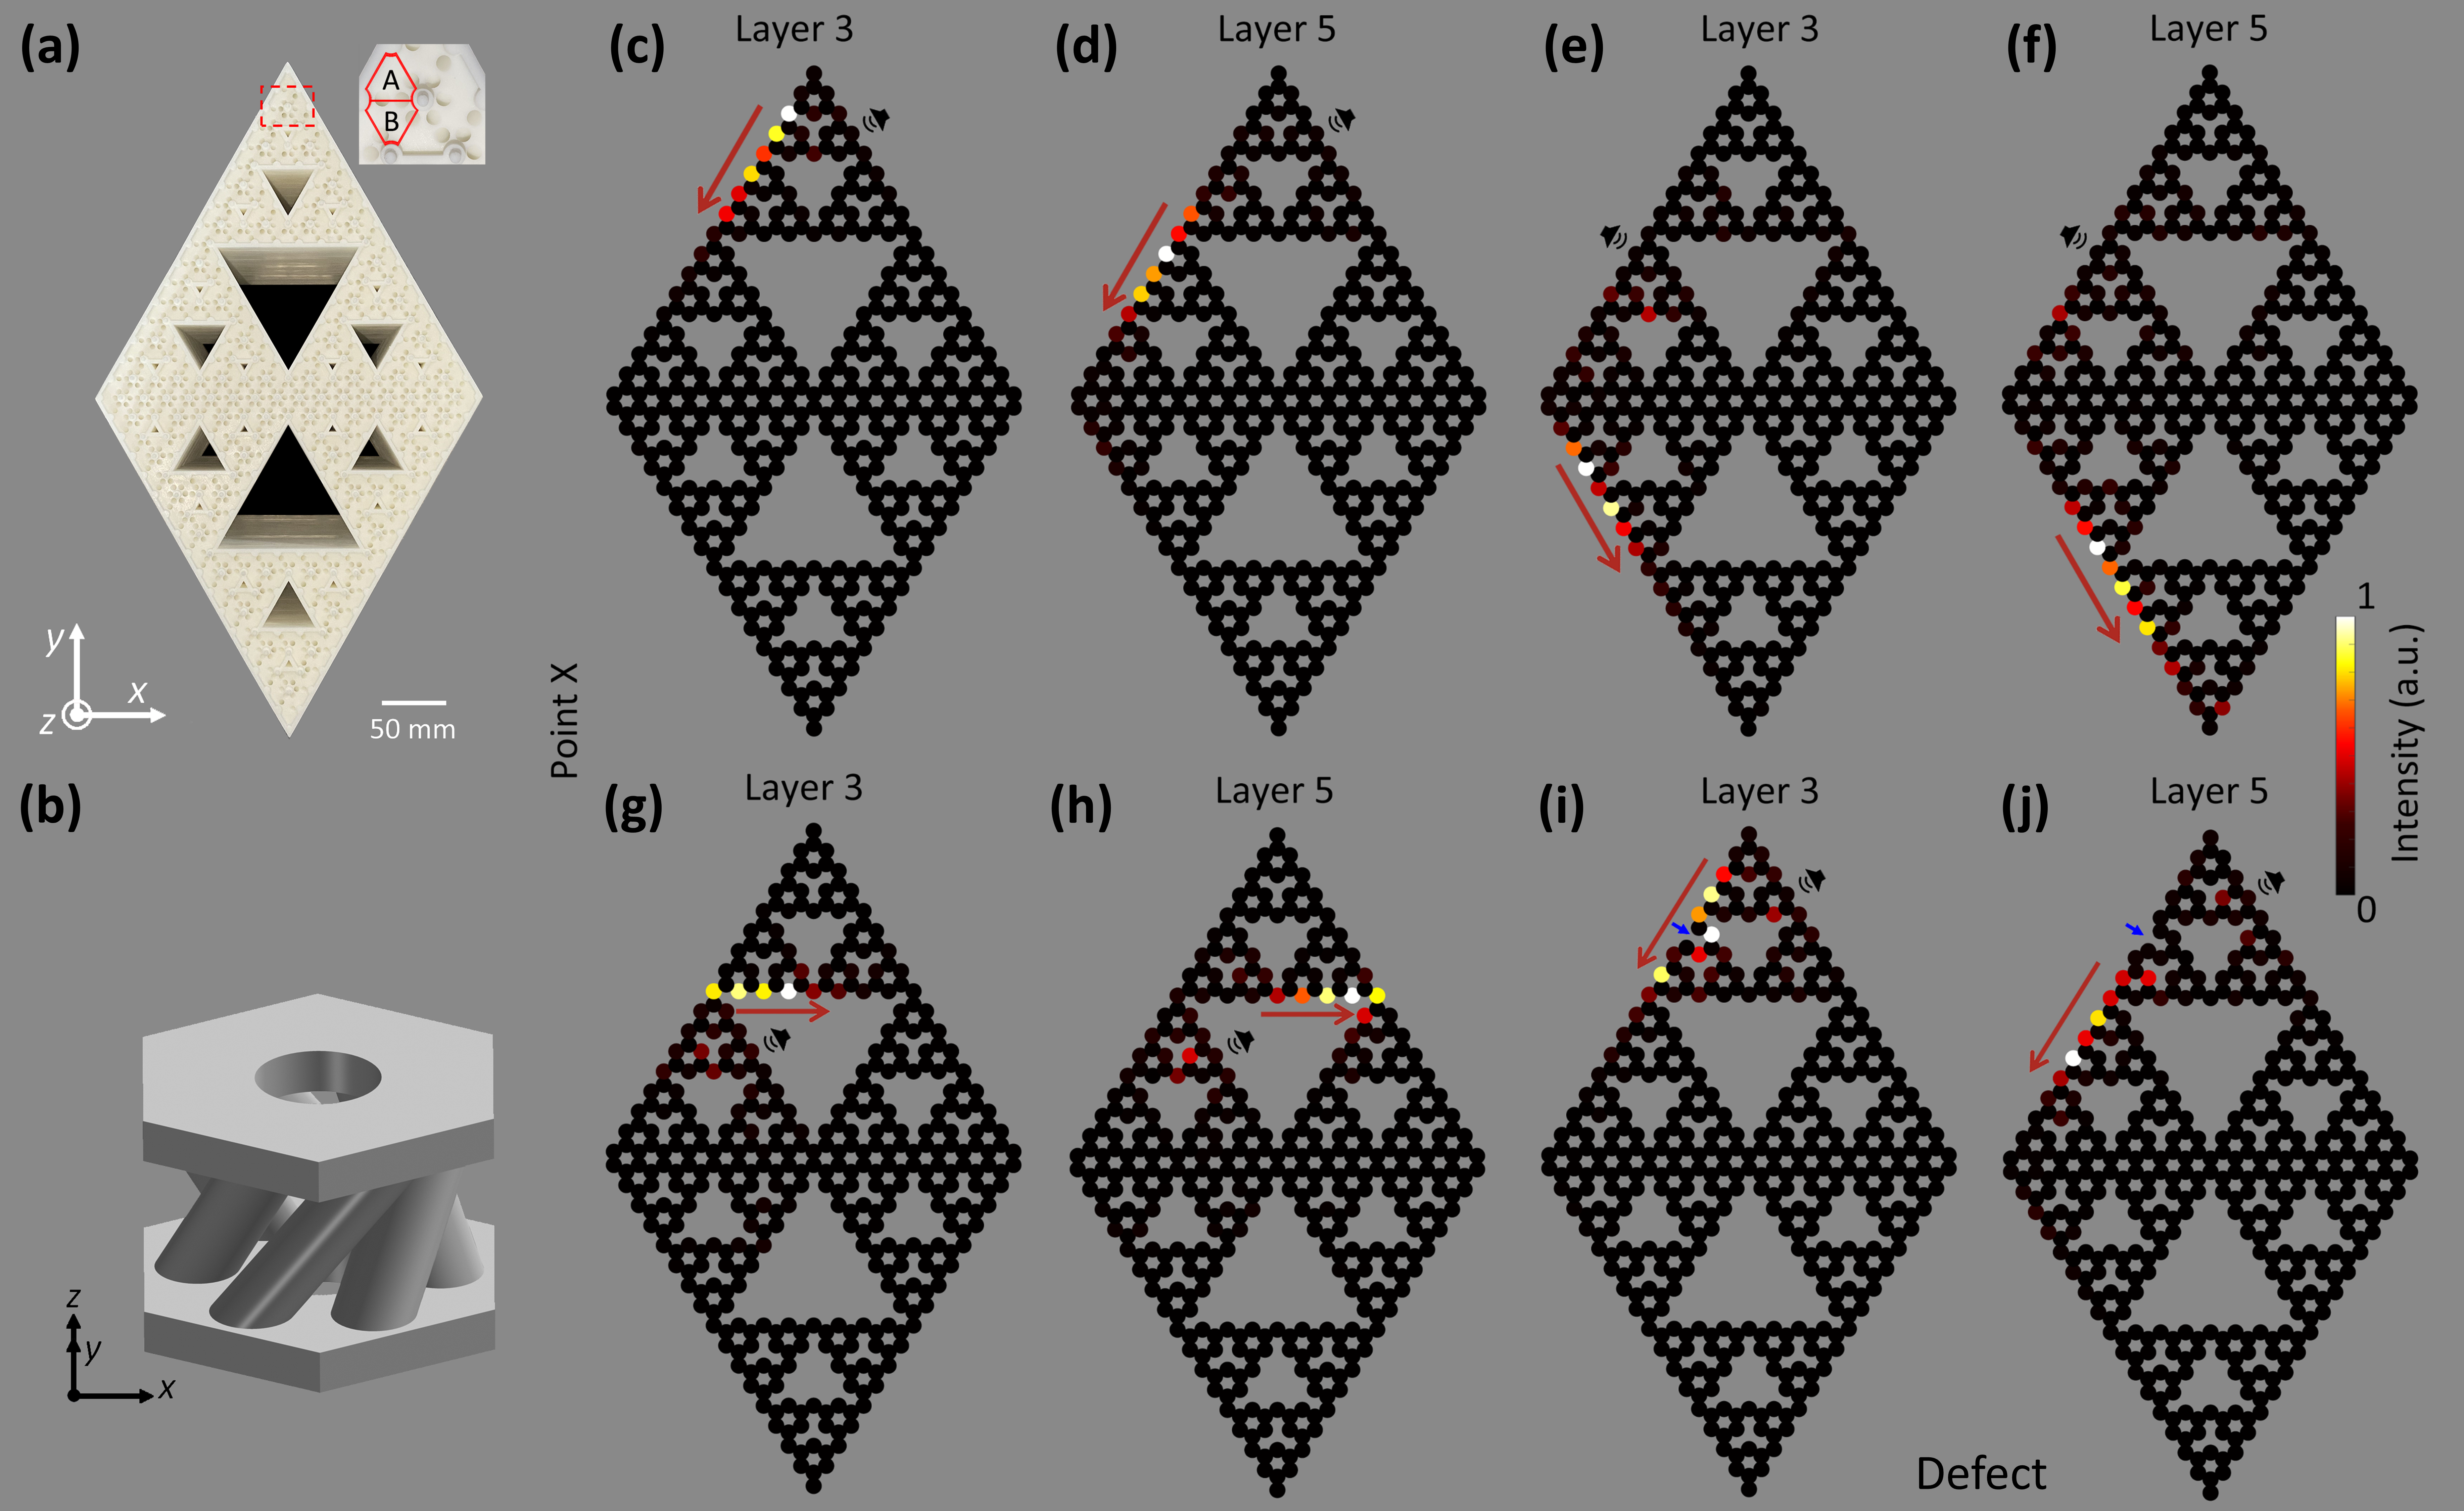
\includegraphics[width=1\linewidth]{figure/FracHaldExp/ExpTopoEdge.png}
    \caption{分形拓扑边界态的观察。(a) 声学样品的照片,插图显示了 A 和 B 亚原子的放大视图。(b) 声学六边形元胞的结构,该结构在 $z$ 轴方向上是周期性的,并可映射到图 1(a) 中的六边形元胞。通过添加手性管道引入复杂的次近邻耦合,并在固定动量 $k_z$ 下包含有效的交错磁通量 [$\phi = k_z d_z \in (0, \pi)$]。(c, d) 外部拓扑边界态在传播 3 层和 5 层后的声强分布。(e, f) 将声源左移,使声波穿过钝角并沿边界进一步向下传播。(g, h) 内部拓扑边界态在传播 3 层和 5 层后的声强分布。(i, j) 在存在缺陷(由蓝色箭头指示)的情况下,边界态在传播 3 层和 5 层后的声强分布。需要注意的是,本图中的拓扑系统对应于无交错势能的结果。红色箭头指示了声波传播的方向。}
    \label{fig:ExpTopoEdge}
\end{figure}

首先,在图\ref{fig:ExpTopoEdge}(c-f) 中,我们展示了不存在交错势能差时($\phi = \pi/2, m=0$) 边界态的拓扑传播情况。示意扬声器指示了声源阵列的位置,该阵列能够发射频率为 11718Hz 的声波,该频率位于拓扑带宽范围 11109Hz 至 11934Hz 内,且具有固定动量 $k_z = \pi/(2d_z)$,表明声波不仅在 $x$-$y$ 平面内传播,还在 $z$ 方向上传播。

经过三层和五层传播后 [图\ref{fig:ExpTopoEdge}(c, d)],我们观察到声波沿外部边界传播,不会渗透到分形晶格的内部,并且在遇到尖角时不会发生后向散射。当将声源左移时,声波穿过钝角并沿边界进一步向下传播,如图\ref{fig:ExpTopoEdge}(e, f) 所示。对于局域于内部边界的边界态,我们也观察到了相同的行为,如图\ref{fig:ExpTopoEdge}(g, h) 所示。需要注意的是,由于声波的损耗特性,声波在每层传播后大约损失 $33\%$ 的能量,并且场强在每一层都被归一化至最大值。

此外,由于拓扑保护,声波应当能够绕过缺陷传播,而不会发生后向散射。我们在图 \ref{fig:ExpTopoEdge}(i, j) 中蓝色箭头所指示的位置封堵了一个空腔,并采用与图\ref{fig:ExpTopoEdge}(c, d) 相同的方法进行实验。可以清楚地观察到,声波沿边界传播,在遇到顶角和缺陷后,继续沿左侧边界向下传播,而没有发生后向散射。我们注意到,在自相似性被破坏的缺陷区域,声波沿着单个亚原子的路径传播,这表明稳健的拓扑传播被推进到了单亚原子尺度。

\subsection{支持边缘态的拓扑带隙}
首先,我们通过紧束缚模拟数值计算了边界态的传输率,结果如图\ref{fig:BandGap}(a) 所示,传输率由最高点归一化。激励源设置在外部边界,可以看到在能量中心 0 处存在一个高传输峰,其对应拓扑边缘态的频率范围。面板 (b, c)为传输峰边缘的时间演化结果,经过20秒的传输,激发态很好的局域在晶格边缘。该高传输带宽内的激励频率导致的传播行为与面板 (b, c) 中所示的行为一致。图\ref{fig:BandGap}(a) 中的灰色阴影区域与数值计算中Bott系数识别的拓扑迁移率隙相对应。传输峰的测量位置为图\ref{fig:BandGap}(b, c) 红色箭头所指位置。

\begin{figure}[htbp]
    \centering
    \includegraphics[width=0.75\linewidth]{figure/FracHaldExp/BandGap.png}
    \caption{支持边界态的拓扑带宽。(a) 通过紧束缚模拟计算边界态的传输率。(b, c) 面板 (a) 中所示点的拓扑传输模拟结果,其中 (b) 对应能量 $-0.46$,(c) 对应能量 $0.46$。(d) 通过实验测得的边界态传输率。(e, f) 在阴影带宽的左侧 (11109Hz) 和右侧 (11934Hz) 处测得的场分布。(e, f) 中的扬声器表示数值模拟和实验中的声源位置。(b, c, e, f) 中的红色箭头表示数值模拟和实验中的接收器位置。}
    \label{fig:BandGap}
\end{figure}

在实验中,我们测量了经过5层传输后的传输率。该传输率定义为声能量在边界处的占比相对于晶格内部的占比,并以频率为变量绘制,如图\ref{fig:BandGap}(d) 所示。我们将半高全宽 (full width at half maximum, FWHM) 视为拓扑带宽,其范围从 11109Hz 到 11934Hz(总计 828Hz)。图\ref{fig:ExpTopoEdge}进行实验时采用的工作频率为 11718Hz,该频率在图 \ref{fig:BandGap}(d) 中由红点标记。实验测得的带宽 [图 \ref{fig:BandGap}(d)] 与有限元模拟计算得到的带宽 [图\ref{fig:AcouFractSpec}(b)] 之间的差异约为 $1\%$。测量格点位置在图\ref{fig:BandGap}(e, f) 中由红色箭头标出。

在半高全宽的边界处测得的场分布如图\ref{fig:BandGap}(e, f) 所示,对应的工作频率分别为 11109Hz 和 11934Hz。从面板 (e) 可以看出,在半高全宽的边缘处,特别是半高全宽的下边缘,声波开始渗透到样品内部。由于每层传播时能量损耗约为 $33\%$,色彩图已归一化至每一层的最大值。

此外,为了进一步验证带隙的存在,我们在实验中观察了频率为 11675Hz 和 11762Hz 的边界态在带隙内的传播情况。如图\ref{fig:BandGap2}所示,即便是对于低频态,激发态在传播三层后仍然很好地局域于边界。
\begin{figure}[htbp]
    \centering
    \includegraphics[width=0.5\linewidth]{figure/FracHaldExp/BandGap2.png}
    \caption{带隙中拓扑状态的观察。(a,b)在阴影带宽靠近左边缘(11109Hz)和靠近右边缘(11934Hz)的工作频率下测量的场分布。}
    \label{fig:BandGap2}
\end{figure}
\subsection{声学分形霍尔丹模型的相变}
分形晶格会产生拓扑相的压缩现象。要想证明这一点,我们需要选择合适的参数,其对应拓扑的二维蜂房晶格,但对应平庸的分形晶格。我们选取参数$\phi = \pi/2, m = 3.6t_2$,也即图\ref{fig:ComsolMass}(a)的Y点。其交错势能项$m = 3.6t_2$小于广为人知的霍尔丹相变边界$m = 3\sqrt{3}t_2$,因此位于霍尔丹模型的拓扑相区域。此时分形晶格的能谱如图\ref{fig:ExpTrivial}(a)所示。通过数值计算,其对应所有态的Bott系数均为零。

\begin{figure}[htbp]
    \centering
    \includegraphics[width=0.85\linewidth]{figure/FracHaldExp/ExpTrivial.png}
    \caption{平庸相中的被困声波。(a) 平庸态的能谱,对应于图 1(c) 中标记的点 Y。(b, c) 声波在传播 5 层后的声强分布,可以明显观察到声波被困。(d) 声波在传播 5 层后的声强分布。相比于图 3(h),可以看到声波无法沿边界传播并绕过拐角。(b-d) 中的示意扬声器表示声源阵列的位置,该阵列发射频率为 10506Hz 的声波。输出声源阵列具有固定动量 $k_z = \pi/(2d_z)$。}
    \label{fig:ExpTrivial}
\end{figure}

在实验中,我们也观察到在平庸点 Y ($\phi = \pi/2, m = 3.6t_2$) 处,声波的传播表现出被困行为。A 和 B 亚晶格之间的格点能量差异 $m$ 是通过简单调整声学空腔的高度引入的,实验参数通过有限元仿真确定。实验采用的工作频率为 10506Hz,且相位阵列仍然维持波矢$k_z=\pi/2d_z$。

笔者首先验证了外边缘的实验结果。声波经过五层传播后,如图\ref{fig:ExpTrivial}(b, c) 所示,当声源从右上边界移动到左下边界时,声波渗透进入样品内部,并在拐角处发生散射。声波受困的结果也在内边缘出现。如图\ref{fig:ExpTrivial}(d) 所示,围绕中心空隙的声波传播同样表现出被困行为,这与图\ref{fig:ExpTopoEdge}(h) 中的结果形成鲜明对比。结合图\ref{fig:ExpTopoEdge}中的实验结果,我们已在实验上验证了将分形晶格引入拓扑 霍尔丹 模型能够保持拓扑相变,同时拓扑相图被压缩。

\section{分形BBH模型的有限元仿真}
\subsection{声学负耦合}
\label{sec:NegCoup}
众所周知,双谐振器系统 [图\ref{fig:NegCoup}(b, d)] 可由两能级哈密顿量描述:
\begin{equation}
    H = \begin{pmatrix} \omega_0 & \pm t \\ \pm t & \omega_0 \end{pmatrix}
\end{equation}
其中,\( t \) 是耦合强度(\( t > 0 \)),\( \omega_0 \) 是单个谐振器中偶极模式的本征频率。通过对角化哈密顿量计算可以发现,无论耦合是正的还是负的,该哈密顿量的本征能量均为 \( \omega_0 \pm t \)。

然而,如图\ref{fig:NegCoup}(a, c) 所示,在正耦合(\( +t \))的情况下,本征矢量为$\psi=\sqrt{2}/2(\pm1,1)^T$。而在负耦合(\( -t \))的情况下,本征矢量为$\psi=\sqrt{2}/2(\mp1,1)^T$。这可以通过采用声学谐振器的偶极模式轻松实现。

如图\ref{fig:NegCoup}(b, d) 所示,我们通过移动谐振器之间的耦合管,实现了正耦合和负耦合。在这两种耦合情况下,右侧谐振器的声压分布保持不变,而左侧谐振器的声压分布相反。因此,我们在声学谐振器系统中实现了正负耦合。此外,改变连接管以形成正耦合和负耦合的方法在先前研究中也被广泛使用\cite{xue2022projectively,li2022acoustic}。

\begin{figure}[htbp]
    \centering
    \includegraphics[width=0.75\linewidth]{figure/HOTIExp/NegCoup.png}
    \caption{紧束缚模型描述耦合声学谐振器。(a, c) 正耦合 (a) 和负耦合 (c) 的紧束缚模型的本征能量与本征态。(b, d) 两个耦合声学谐振器的本征频率和本征模式。连接的谐振器被分裂为高低本征频率,分别为 2209.5 Hz 和 2056.1 Hz。}
    \label{fig:NegCoup}
\end{figure}
\subsection{声学BBH模型原胞}
能带拓扑系统中的带隙演化是表征拓扑物态的核心判据。根据拓扑能带理论\cite{hasan2010colloquium},拓扑相变的本质在于系统全局拓扑数的改变,这一过程通常伴随能带结构的闭合-重开现象。基于第\ref{sec:NegCoup}节建立的声学负耦合实现方案,在本节,我们将计算两种不同模式下的声学频带,一种是具有全正耦合的单极模式,另一种一种是具有负耦合的偶极模式,系统研究其能带拓扑特性。特别地,通过调节耦合参数观测到负耦合模式下拓扑带隙的闭合过程,为体系的拓扑相变提供了直接证据。

图 \ref{fig:EnergyBand}(a) 展示了 BBH 模型的声学原胞结构。其中,蓝色的长方形声腔代表原胞的格点,红色和绿色的连接腔分别对应正耦合与负耦合通道。耦合强度可通过调节声腔横截面的大小进行控制。由于负耦合的存在,原胞内会积累 $\pi$ 相位流,从而影响能带结构。

\begin{figure}[htbp]
    \centering
    \includegraphics[width=0.85\linewidth]{figure/HOTIExp/EnergyBand.png}
    \caption{声学高阶拓扑绝缘体的原胞结构与能带特征。(a) BBH 模型声学原胞示意图,蓝色矩形腔为晶格节点,红/绿连接管分别对应正/负耦合;(b) 单极模式对应的二维 SSH 模型能带,显示$\Gamma$点处体态简并;(c) 偶极模式下的拓扑非平庸能带,中心区域出现特征带隙。}
    \label{fig:EnergyBand}
\end{figure}

对于该系统,当激发单极振动模式时,所有的耦合均为正耦合。这使得系统等效于二维 SSH(Su-Schrieffer-Heeger)模型\cite{zheng2022observation}。在该情况下,系统的高对称点频带结构如图 \ref{fig:EnergyBand}(b) 所示。在频谱中心,两条体带带隙关闭,且在高对称点$\Gamma(0,0)$处出现简并态。

引入负耦合后激发偶极模式与单极模式形成鲜明对比,体系展现出显著不同的能带结构。 如图 \ref{fig:EnergyBand}(c) 所示。在该模式下,频带中心出现约$\Delta f = 286.2$ Hz的拓扑带隙。该带隙对应实空间中的拓扑局域态,满足高阶体-边对应关系\cite{benalcazar2017quantized}。

为了进一步揭示 其拓扑相变性质,笔者计算了能带K点处不同胞内/胞间耦合比$t_1/t_2$的特征频率[图\ref{fig:GapClosing}]。在本节中,耦合管道横截面是正方形,其中胞外耦合管道横截面的边长为$L=8$毫米。我们定义胞内胞外耦合比$t_1/t_2$为胞内胞外横截面边长的比例。如图\ref{fig:GapClosing}所示,当$t_1/t_2$从0.1增至1时,带隙宽度满足
\begin{equation}
    \Delta(t)\propto |1 - t_1/t_2|
\end{equation}
最终在临界点$t_1/t_2=1$处实现带隙闭合,形成具有线性色散关系的狄拉克锥。这一连续相变过程证实体系存在两种拓扑相,其分界由带隙闭合条件$t_1 = t_2$决定。
\begin{figure}[htbp]
    \centering
    \includegraphics[width=0.5\linewidth]{figure/HOTIExp/GapClosing.png}
    \caption{频带带隙关闭。}
    \label{fig:GapClosing}
\end{figure}

为了进一步展示拓扑相变的结果,笔者继续计算了在y方向选取开边界,但在x方向选取周期性边界条件的结果。结果如图\ref{fig:OBCPBC}所示,图\ref{fig:OBCPBC}(a)展示了相变点处($t_1=t_2$)时的结果,上下频带简并,频隙闭合,导致平庸的拓扑。而图\ref{fig:OBCPBC}(b)则展示了处于前文拓扑时的结果,此时上下两带被打开一个拓扑带隙,中间出现了红色标记的拓扑局域态。拓扑局域态局域在y方向开边界的两边,如图\ref{fig:OBCPBC}(c)所示。拓扑局域态选取$k_x=0$的结果,此时分布于上下两边的局域态特征频率分别为$5698.8$Hz和$5668.8$Hz

\begin{figure}[htbp]
    \centering
    \includegraphics[width=0.65\linewidth]{figure/HOTIExp/OBCPBC.jpg}
    \caption{拓扑带隙内的拓扑局域态。(a) 拓扑相变点结果,此时能带闭合。(b) 拓扑能带结构。此时能带打开一个带隙,中间出现红色标记的拓扑局域态。(c) 拓扑局域态的声学模式分布图。} 
    \label{fig:OBCPBC}
\end{figure}
\subsection{声学分形晶格频谱}
\label{sec:fractal_states}
通过优化胞内/胞间耦合比至$t_1/t_2=0.13$,体系拓扑带隙显著扩展至$\Delta f=494.4\ \mathrm{Hz}$。图\ref{fig:ComsolWholeLat}(a)展示了该参数下的完整频谱结构,其局域态分布呈现出多层级拓扑特征。通过分析不同特征频率的声压分布,获得不同空间尺度的角态分布规律。观察该频谱,可以发现其关于频谱中心的对称性被打破。这表明其手性对称性破缺。这种破缺原因可能来自于强胞间耦合诱发了同子晶格格点之间的次近邻耦合以及子晶格势能。次近邻耦合和子晶格势能会打破晶格的手性对称性。

\begin{figure}[htbp]
    \centering
    \includegraphics[width=0.9\linewidth]{figure/HOTIExp/ComsolWholeLat.png}
    \caption{分形晶格的多级拓扑态分布。 (a) $t_1/t_2=0.13$时的频谱结构(红/黄/青/蓝点分别对应外角态、A类内角态、B类内角态和边缘态)。 
    (b) 外角态的波函数分布。
    (c,d) 内角态A/B的空间局域化特征,对应不同层级分形结构的$3\pi/2$夹角区域。
     (e) 一维边缘态的波函数分布。}
    \label{fig:ComsolWholeLat}
\end{figure}

作为手性对称性破缺的结果,频谱中心附近的外角态(红点)不再满足四重简并关系,外角态出现于频率5357.5Hz到5360.4Hz范围内。其波函数分布可由分形边界条件推导:
\begin{equation}
    \psi_n(r) \propto e^{-r/\xi}\cos\left(\frac{n\pi}{2}\theta\right),\quad n=1,3,5,7
\end{equation}
其中$\xi=1/\ln(t_2/t_1)$为局域长度,$\theta\in[0,2\pi)$为角向坐标。如图\ref{fig:ComsolWholeLat}(b)所示,这些态严格局域在晶格四个外角区域,其$\pi/2$夹角与传统高阶拓扑绝缘体的角态一致。图中展示的态对应于5326.8Hz的特征频率。

在能隙$\Delta f$范围内,我们观察到两类内角态(黄/青色点)。A类态(黄点):局域在$G(2)$级分形结构的4个内角,满足$3\pi/2$开口角条件。B类态(青点):分布于$G(1))$级分形结构的32个内角。其中,A类内角态出现于特征频率5347.5Hz到5356.2Hz范围内;B类内角态出现于特征频率5203.2Hz到5375Hz范围内。图\ref{fig:ComsolWholeLat}(c,d)展示了分别展示了AB两类内角态的示例,其对应特征频率分别为5209.3Hz和5326.9Hz。由于内角态局域在内部空洞,这导致内角态分裂为两个相邻边缘位置,这与传统高阶拓扑绝缘体的角态局域化机制有本质区别。

最后,笔者绘制了声学分形晶格的边缘态分布,如图\ref{fig:ComsolWholeLat}(e)所示。边缘态出现于频率5013.4Hz到5080.3Hz的下频谱范围,以及5574.7Hz到5638.5Hz的上频谱范围内。与先前的理论结果一致,分形晶格的边缘态既出现于外边缘,也出现与内边缘。图\ref{fig:ComsolWholeLat}(e)只展示了外边缘态结果。


\subsection{G(1)声学分形晶格频谱与场分布}
前文展示了G(2)代的声学谢宾斯基地毯高阶拓扑绝缘体的能谱与拓扑态分布。接下来笔者将证明高阶拓扑态在不同迭代的声学分形晶格中都能稳定存在。图\ref{fig:G1}(a)为 数值模拟的 G(1) 代谢宾斯基地毯高阶拓扑声学超材料的本征频率,其中 \( t_1 < t_2 \)。内角态、外角态和边缘态分别用黄色、红色和蓝色点表示。(b)-(d) 不同模式的模拟声压场分布,包括外角态 (5359.4 Hz)、内角态 (5326.4 Hz)、边缘态 (5876.1 Hz)。

\begin{figure}[htbp]
    \centering
    \includegraphics[width=0.5\linewidth]{figure/HOTIExp/G1.png}
    \caption{G(1)声学分形晶格频谱与场分布}
    \label{fig:G1}
\end{figure}

由于在G(1)代的声学谢宾斯基地毯晶格中不存在体格点,其一个独特的拓扑性质是其频谱不存在体态。在前文的谢宾斯基三角形霍尔丹模型中,晶格亦不存在体格点,但晶格仍存在体态。这是由于一阶拓扑绝缘体的拓扑相变依赖体能带的关闭再打开。而高阶拓扑绝缘体的拓扑相变可以在体带隙维持打开,而仅通过边缘哈密顿量的带隙闭合再开启来产生\cite{ezawa2020edge,khalaf2021boundary}。因此分形晶格拓扑角态的出现并不依赖于体态,这导致了在没有对应体格点的分形晶格中,不再存在体态。

我们模拟了 G(1) 代谢宾斯基地毯分形声学超材料的本征频率和本征态,在 \( t_1 \neq t_2 \) 的情况下。当 \( d_1 = 3.2 \) mm 和 \( d_2 = 8 \) mm(\( t_1 < t_2 \))时,谢宾斯基地毯 G(1) 的频谱如图\ref{fig:G1}(a) 所示。其中,存在 4 个外角态(红色点)、16 个边缘态(蓝色点)和 12 个内角态(黄色点),分别对应于单体、二聚体和三聚体的共振腔总数。从另一个角度来看, G(1) 代谢宾斯基地毯中不存在四聚体,因此没有体态。模拟得到的声压场分布表明,外角态 (5359.4 Hz)、内角态 (5326.4 Hz)、边缘态 (5876.1 Hz)的声学能量均强烈局域于相应的共振腔。

\section{声学分形BBH模型的观测}
\subsection{实验装置}
\label{sec:experimental_setup}
实验样品采用高精度3D打印技术制备,如图\ref{fig:ExperimentalSetup}所示。样品选用光敏树脂材料(杨氏模量$E=2.5$ GPa,密度$\rho=1.15$ g/cm$^3$)以确保结构稳定性。单个共振器中的空气腔体尺寸为 \( 32 \text{mm} \times 16 \text{mm} \times 16 \text{mm} \),包围壁的厚度为 2mm。在共振器的两侧分别留有一个 \( 4 \text{mm} \times 3 \text{mm} \) 的方形孔和一个半径为 1.5mm 的圆形孔,分别用于输入和输出声学信号。两个共振器通过一根长度为 16mm 的管道相连,其垂直截面尺寸分别为 \( 3.2 \text{mm} \times 3.2 \text{mm} \)(用于站点内跃迁)和 \( 3.2 \text{mm} \times 8 \text{mm} \)(用于站点间跃迁)。

\begin{figure}[htbp]
    \centering
    \includegraphics[width=0.5\linewidth]{figure/HOTIExp/ExperimentalSetup.png}
    \caption{声学拓扑实验装置示意图}
    \label{fig:ExperimentalSetup}
\end{figure}

图\ref{fig:ExperimentalSetup}显示了实验装置的示意图。在测量过程中,我们将扬声器(Knowles SWFK-31736-000,大小$5.00mm \times 2.73mm \times 1.4mm$)插入共振器的方形小孔作为激励源。扬声器频响范围200Hz-7.6kHz,阻抗7Ohms,灵敏度97dBA。并将麦克风(Brüel Kjær 4187)插入圆形小孔作为检测探头。麦克风频响范围1Hz-20kHz,动态范围42 – 164 dB,压强系数-0.007 dB/kPa,灵敏度3.16 mV/Pa。该探针麦克风计算机通过数据分析仪(Brüel Kjær 3160-A-042)记录每个站点的声压数据。 数据分析仪通过TCP/IP协议栈中的网络接口连接到计算机。
\subsection{声学局域态密度}
\label{sec:LDOS}
LDOS表征体系对特定频率声波的态响应能力\cite{landi2018acoustic}。考虑位于$r_0$的单极子声源,其声压场$p(r,t)$满足非齐次波动方程
\begin{equation}
    \nabla^2 p(r,t) - \frac{1}{c_0^2} \frac{\partial^2 p(r,t)}{\partial t^2} = -\rho_0 \frac{\partial Q(t)}{\partial t} \delta(r - r_0)
\end{equation}
其中$c_0=343\ \mathrm{m/s}$为空气声速,$\rho_0=1.29\ \mathrm{kg/m^3}$为空气密度,$Q(t)=Q_0 e^{-i\omega t}$为声源强度。引入时谐条件$p(r,t)=p(r)e^{-i\omega t}$,可得
\begin{equation}
    (\nabla^2 + k^2)p(r) = i\omega\rho_0 Q_0 \delta(r - r_0)
    \label{eq:Helmholtz}
\end{equation}
其中波数$k=\omega/c_0$。

定义格林函数$G(\omega,r,r_0)$满足:
\begin{equation}
    (\nabla^2 + k^2)G(\omega,r,r_0) = \delta(r - r_0)
    \label{eq:Green}
\end{equation}
比较方程(\ref{eq:Helmholtz})与(\ref{eq:Green}),可得声压场解:
\begin{equation}
    p(r) = i\omega\rho_0 Q_0 G(\omega,r,r_0)
    \label{eq:pressure}
\end{equation}

在经典系统中,位置r处的LDOS可以写作\cite{sheng2007introduction}:
\begin{equation}
    \rho(\omega,r) = -\frac{2\omega}{\pi c_0^2} \mathrm{Im}\{G(\omega,r,r_0)\}
    \label{eq:LDOS_def}
\end{equation}
联立方程(\ref{eq:pressure})与(\ref{eq:LDOS_def}),可得声压与LDOS的定量关系:
\begin{equation}
    \mathrm{Re}[p(r)] = \frac{\pi c_0^2 \rho_0 Q_0}{2\omega} \rho(\omega,r)
    \label{eq:measurement}
\end{equation}
该式表明,测量声压正比于体系的LDOS分布。

\subsection{拓扑态的实验观测}
为了在实验上验证分形系统中的高阶拓扑相,我们设计并制造了由声学共振器组成的声学分形晶格,采用直接 3D 打印技术。实验中真实结构的照片如图\ref{fig:ExpMeas}(a) 所示。晶格参数选择依据第\ref{sec:fractal_states}节理论预测,固定耦合比$t_1/t_2=0.13$以实现最大带隙$\Delta f=494.4\ \mathrm{Hz}$。每个晶格节点对应尺寸为$32\ \mathrm{mm}\times16\ \mathrm{mm}\times16\ \mathrm{mm}$的声学共振腔,耦合管道参数如第\ref{sec:experimental_setup}节所述。
\begin{figure}[htbp]
    \centering
    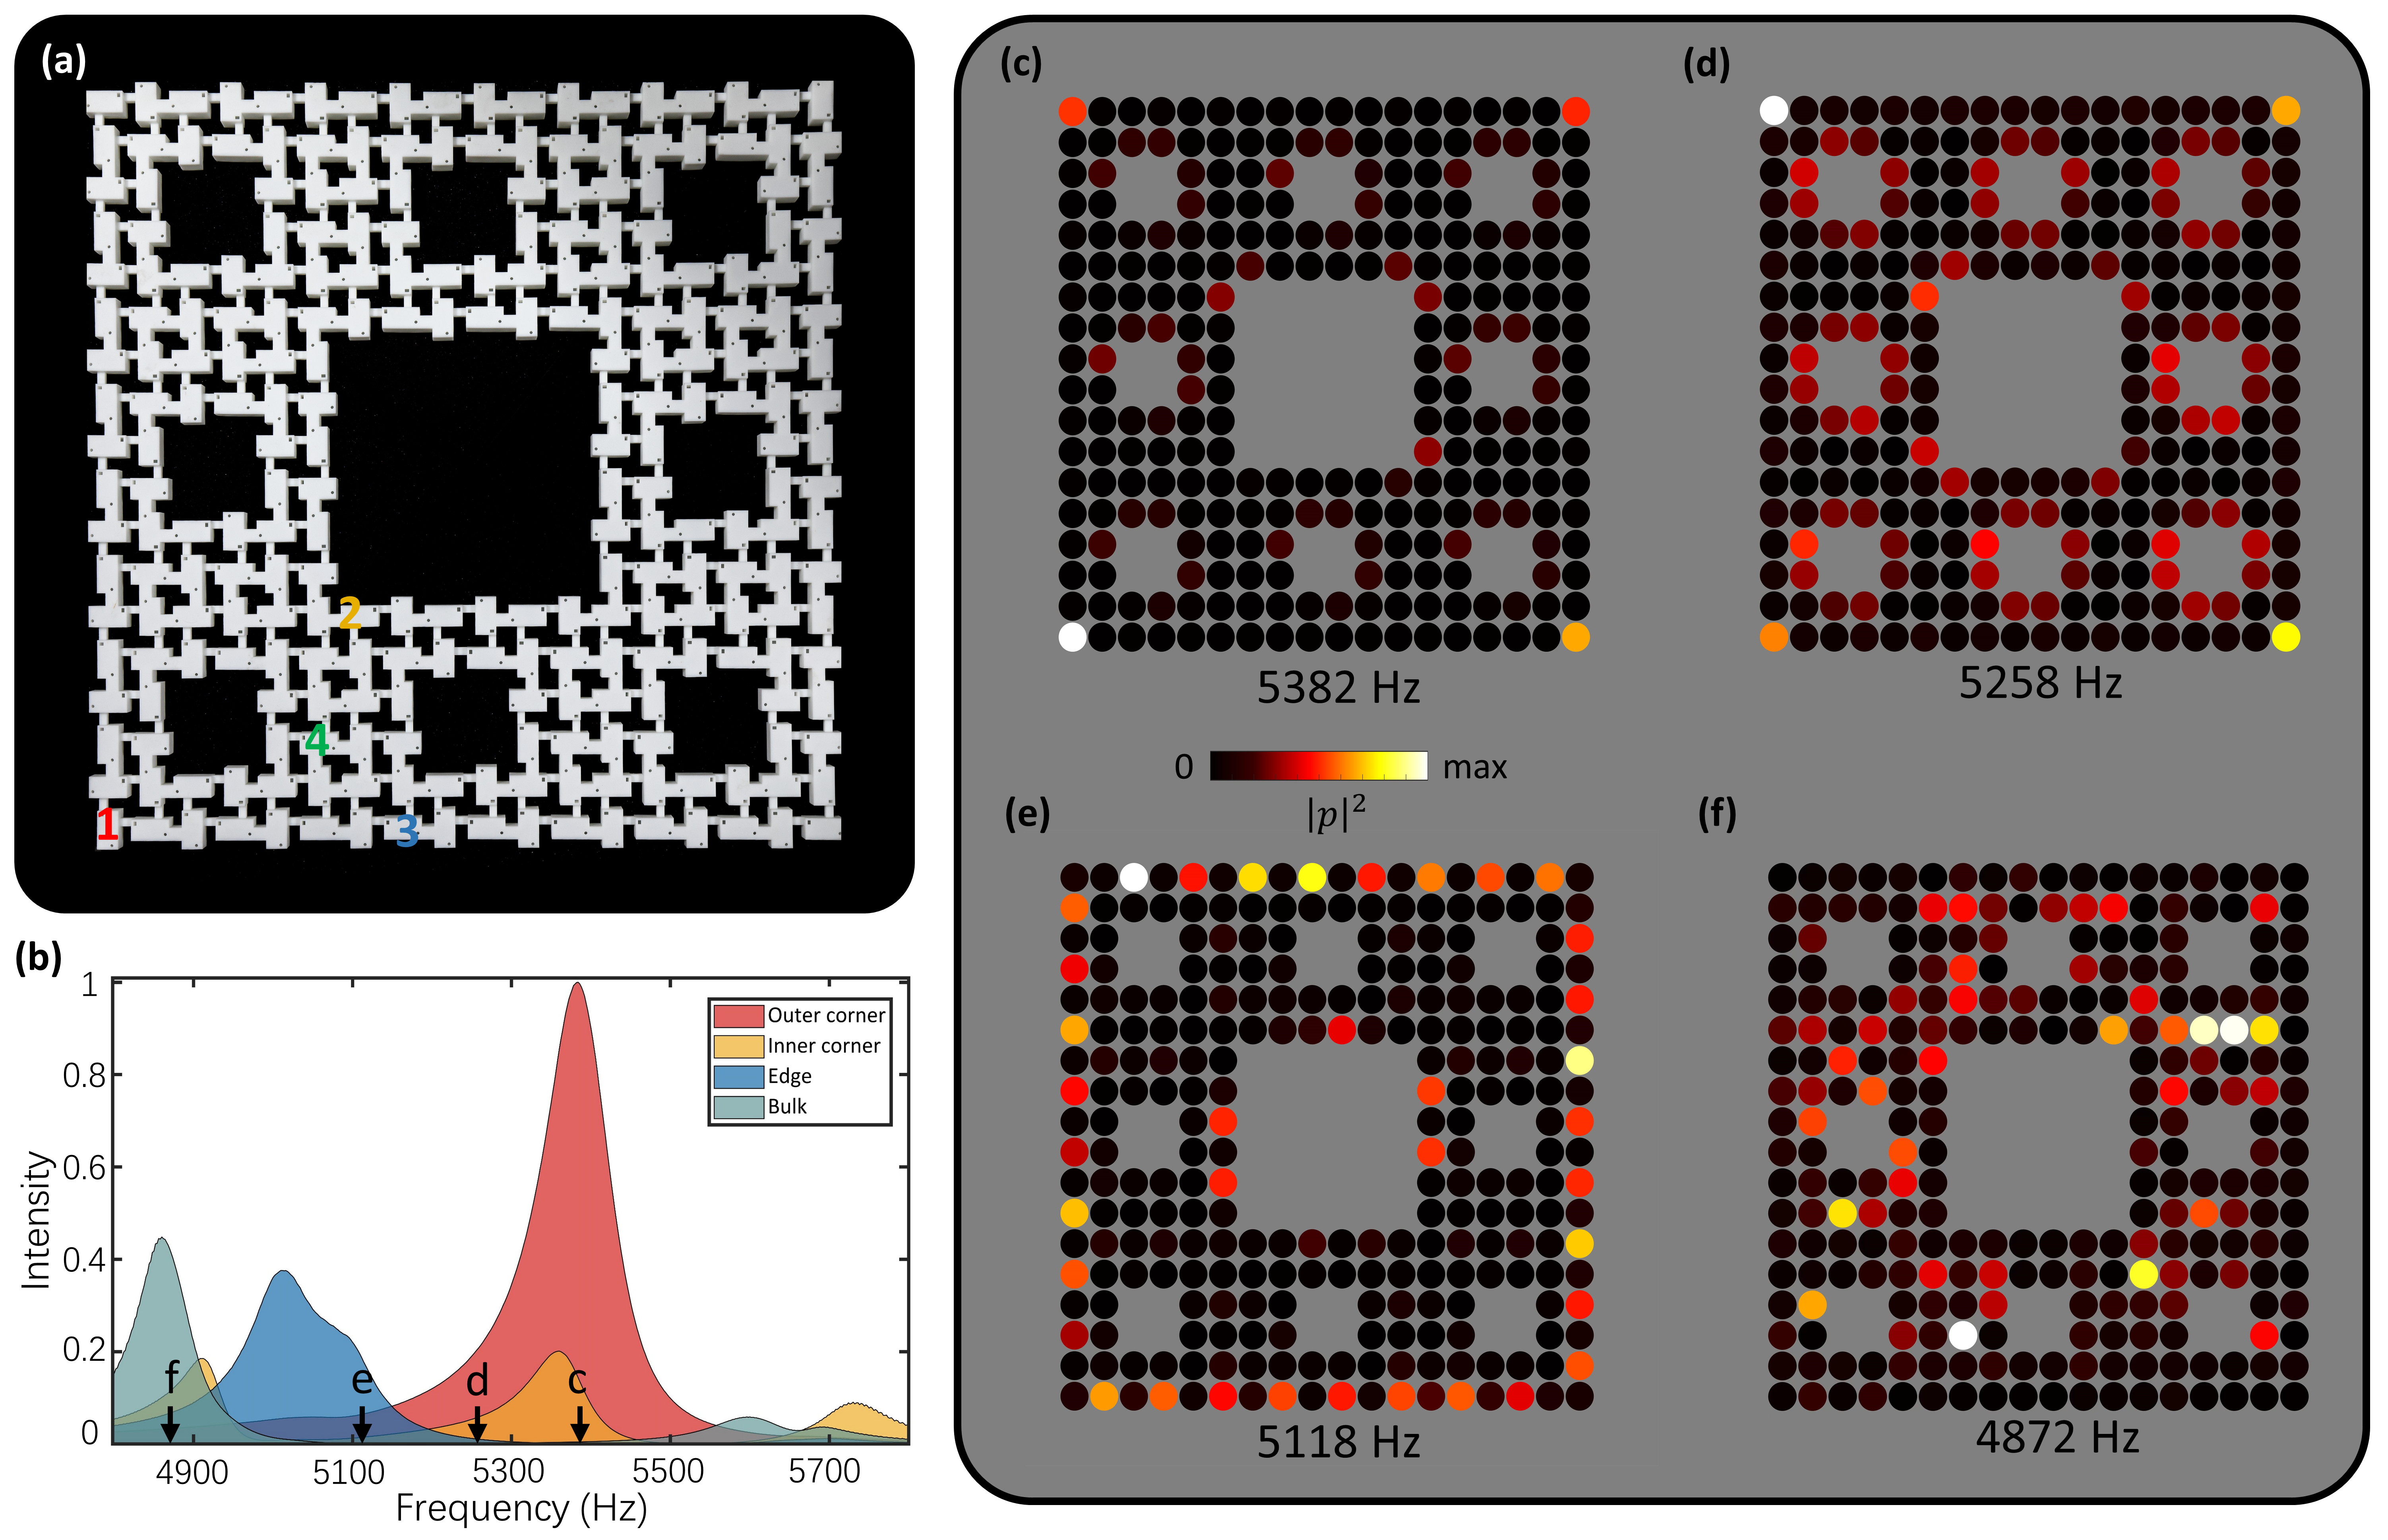
\includegraphics[width=1\linewidth]{figure/HOTIExp/ExpMeas.png}
    \caption{实验观测声学分形晶格中的高阶拓扑绝缘体。(a) 实验样品的照片。(b) 在外角、内角、边缘和“体”站点测得的局部态密度,对应于 (a) 中标记的 ‘1’、‘2’、‘3’ 和 ‘4’,分别用红色、黄色、蓝色和绿色表示。(c-f) 分别在 5382 Hz、5258 Hz、5118 Hz 和 4872 Hz 频率下的强度分布,对应于外角态、内角态、边缘态和“体”态。}
    \label{fig:ExpMeas}
\end{figure}
在实验中,扬声器通过共振器一侧的方形小孔插入样品,产生声波。同时,麦克风插入共振器另一侧的圆形小孔,用于采集响应数据,这些数据可视为局部态密度[详细内容见第\ref{sec:LDOS}节]。该测量遍及样品的所有共振器,以获取声场分布。

在图\ref{fig:ExpMeas}(b) 中,我们展示了位于外角、内角、边缘和“体”站点(分别标记为 1、2、3、4)的四个共振器的测量强度谱。体态的响应谱(绿色曲线)呈现双峰结构,中心频率分别为 $4872 Hz$ 和 $5674 Hz$,表明两峰之间存在宽频隙,间隔$\Delta f=802\ \mathrm{Hz}$。外角态的响应强度(红色曲线)在带隙中心$f_c=5382\ \mathrm{Hz}$处出现尖锐峰。而内角态的响应强度(黄色曲线)分布在频隙和“体”频率范围内,这与三聚体基态与四聚体基态的混合相一致。需要注意的是,由于$t_2$耦合的管道较粗,带来了子晶格势能,系统的手性对称性被破坏,导致边缘态的响应强度(蓝色曲线)主要分布在红色曲线的一侧。

为了验证子晶格势能的影响,笔者对声学原胞在周期性边界条件下的模拟频带如图 \ref{fig:mass}(a) 所示。在模拟中,站点内(站点间)跃迁分别为 40.1 Hz 和 299 Hz,满足正文中的 \( t_1/t_2 = 0.13 \)。不同于紧束缚模型 [见图 \ref{fig:mass}(b)],由于引入了胞间管道,原本“体”态的简并被打破,这意味着系统不再保持手性对称性。

\begin{figure}[htbp]
    \centering
    \includegraphics[width=0.5\linewidth]{figure/HOTIExp/mass.png}
    \caption{子晶格质量项。(a) 声学晶格的模拟频带色散关系。(b, c) 分别为未引入和已引入相反现场势能的紧束缚模型计算得到的频带色散关系。(d) 边缘态的总概率分布。}
    \label{fig:mass}
\end{figure}

这一分裂效应可以通过在对角站点引入相反的势能来解释,如图\ref{fig:mass}(c) 所示。因此,边缘态的总概率不再均匀分布在边界上,如图\ref{fig:mass}(d) 所示。此外,势能会将“体”态驱动至边缘态,从而导致边缘态与“体”态的频率范围相互重叠,并且所显示的边缘态在晶格的“体”区域也存在分布。计算结果与图\ref{fig:ExpMeas}(e) 中的实验测得边缘态强度分布高度一致。

为了进一步验证分形模型中的高阶拓扑绝缘体,利用扫描式声压测量获得了外角态、内角态、边缘态和“体”态的空间场分布,并将结果绘制在图\ref{fig:ExpMeas}(c–f) 中。从图\ref{fig:ExpMeas}(c) 可以清晰地看到,在 $5382 Hz$ 的固定频率下,声学强度主要局域在四个外角,这是传统高阶拓扑绝缘体的重要特征。而在略低于外角态峰值的 $5258 Hz$ 频率处,声学强度分布在不同的内角,如图\ref{fig:ExpMeas}(d) 所示,展现出自相似性和分数维特性。需要注意的是,由于本征态的频率范围较小,外角态与内角态的场分布存在一定的重叠。

相比之下,在边缘态 (e) 和“体”态 (f) 处,声学强度主要分布在蓝色和灰色曲线对应的频率范围内。如图\ref{fig:ExpMeas}(e) 所示,边缘态的场强度呈现出离散分布,这是由于声学晶格制造过程中的限制。这些实验结果与数值模拟高度一致。

\subsection{实验频谱与仿真频谱的对应}
为了验证模拟结果与实验结果的一致性,我们在图\ref{fig:Comparation}(a) 中绘制了声学晶格的模拟频谱。红色和黄色点分别表示外角态和内角态。由于边缘态与“体”态存在重叠,我们将边缘态和“体”态均用灰色点表示。测得的强度谱如图 \ref{fig:Comparation}(b) 所示,红色、黄色、蓝色和绿色区域分别对应于在外角态、内角态、边缘态和“体”站点测得的强度谱。图\ref{fig:Comparation}(b) 中的实验结果与图\ref{fig:Comparation}(a) 中的模拟结果高度一致。
\begin{figure}[htbp]
    \centering
    \includegraphics[width=0.75\linewidth]{figure/HOTIExp/Comparation.png}
    \caption{模拟结果与实验结果的对比。(a) 声学晶格的模拟频谱。红色、黄色和灰色点分别表示外角态、内角态和边缘/“体”态。(b) 测得的强度谱。红色、黄色、蓝色和绿色区域分别表示在外角、内角、边缘和“体”站点测得的强度谱。}
    \label{fig:Comparation}
\end{figure}